\documentclass[12pt]{article}
\usepackage[left=0.5in,right=0.5in,top=0.5in,left=0.5in]{geometry}
\usepackage{algpseudocode}
\usepackage{algorithm}
\usepackage{circuitikz}
\usepackage{amsfonts}
\usepackage{amsmath}

\title{\textsc{Homework 2}}
\author{Henry Trinh}

\begin{document}
\maketitle

\newpage % PROBLEM 1 %
\section*{Problem 1}
\subsection*{Part 1}
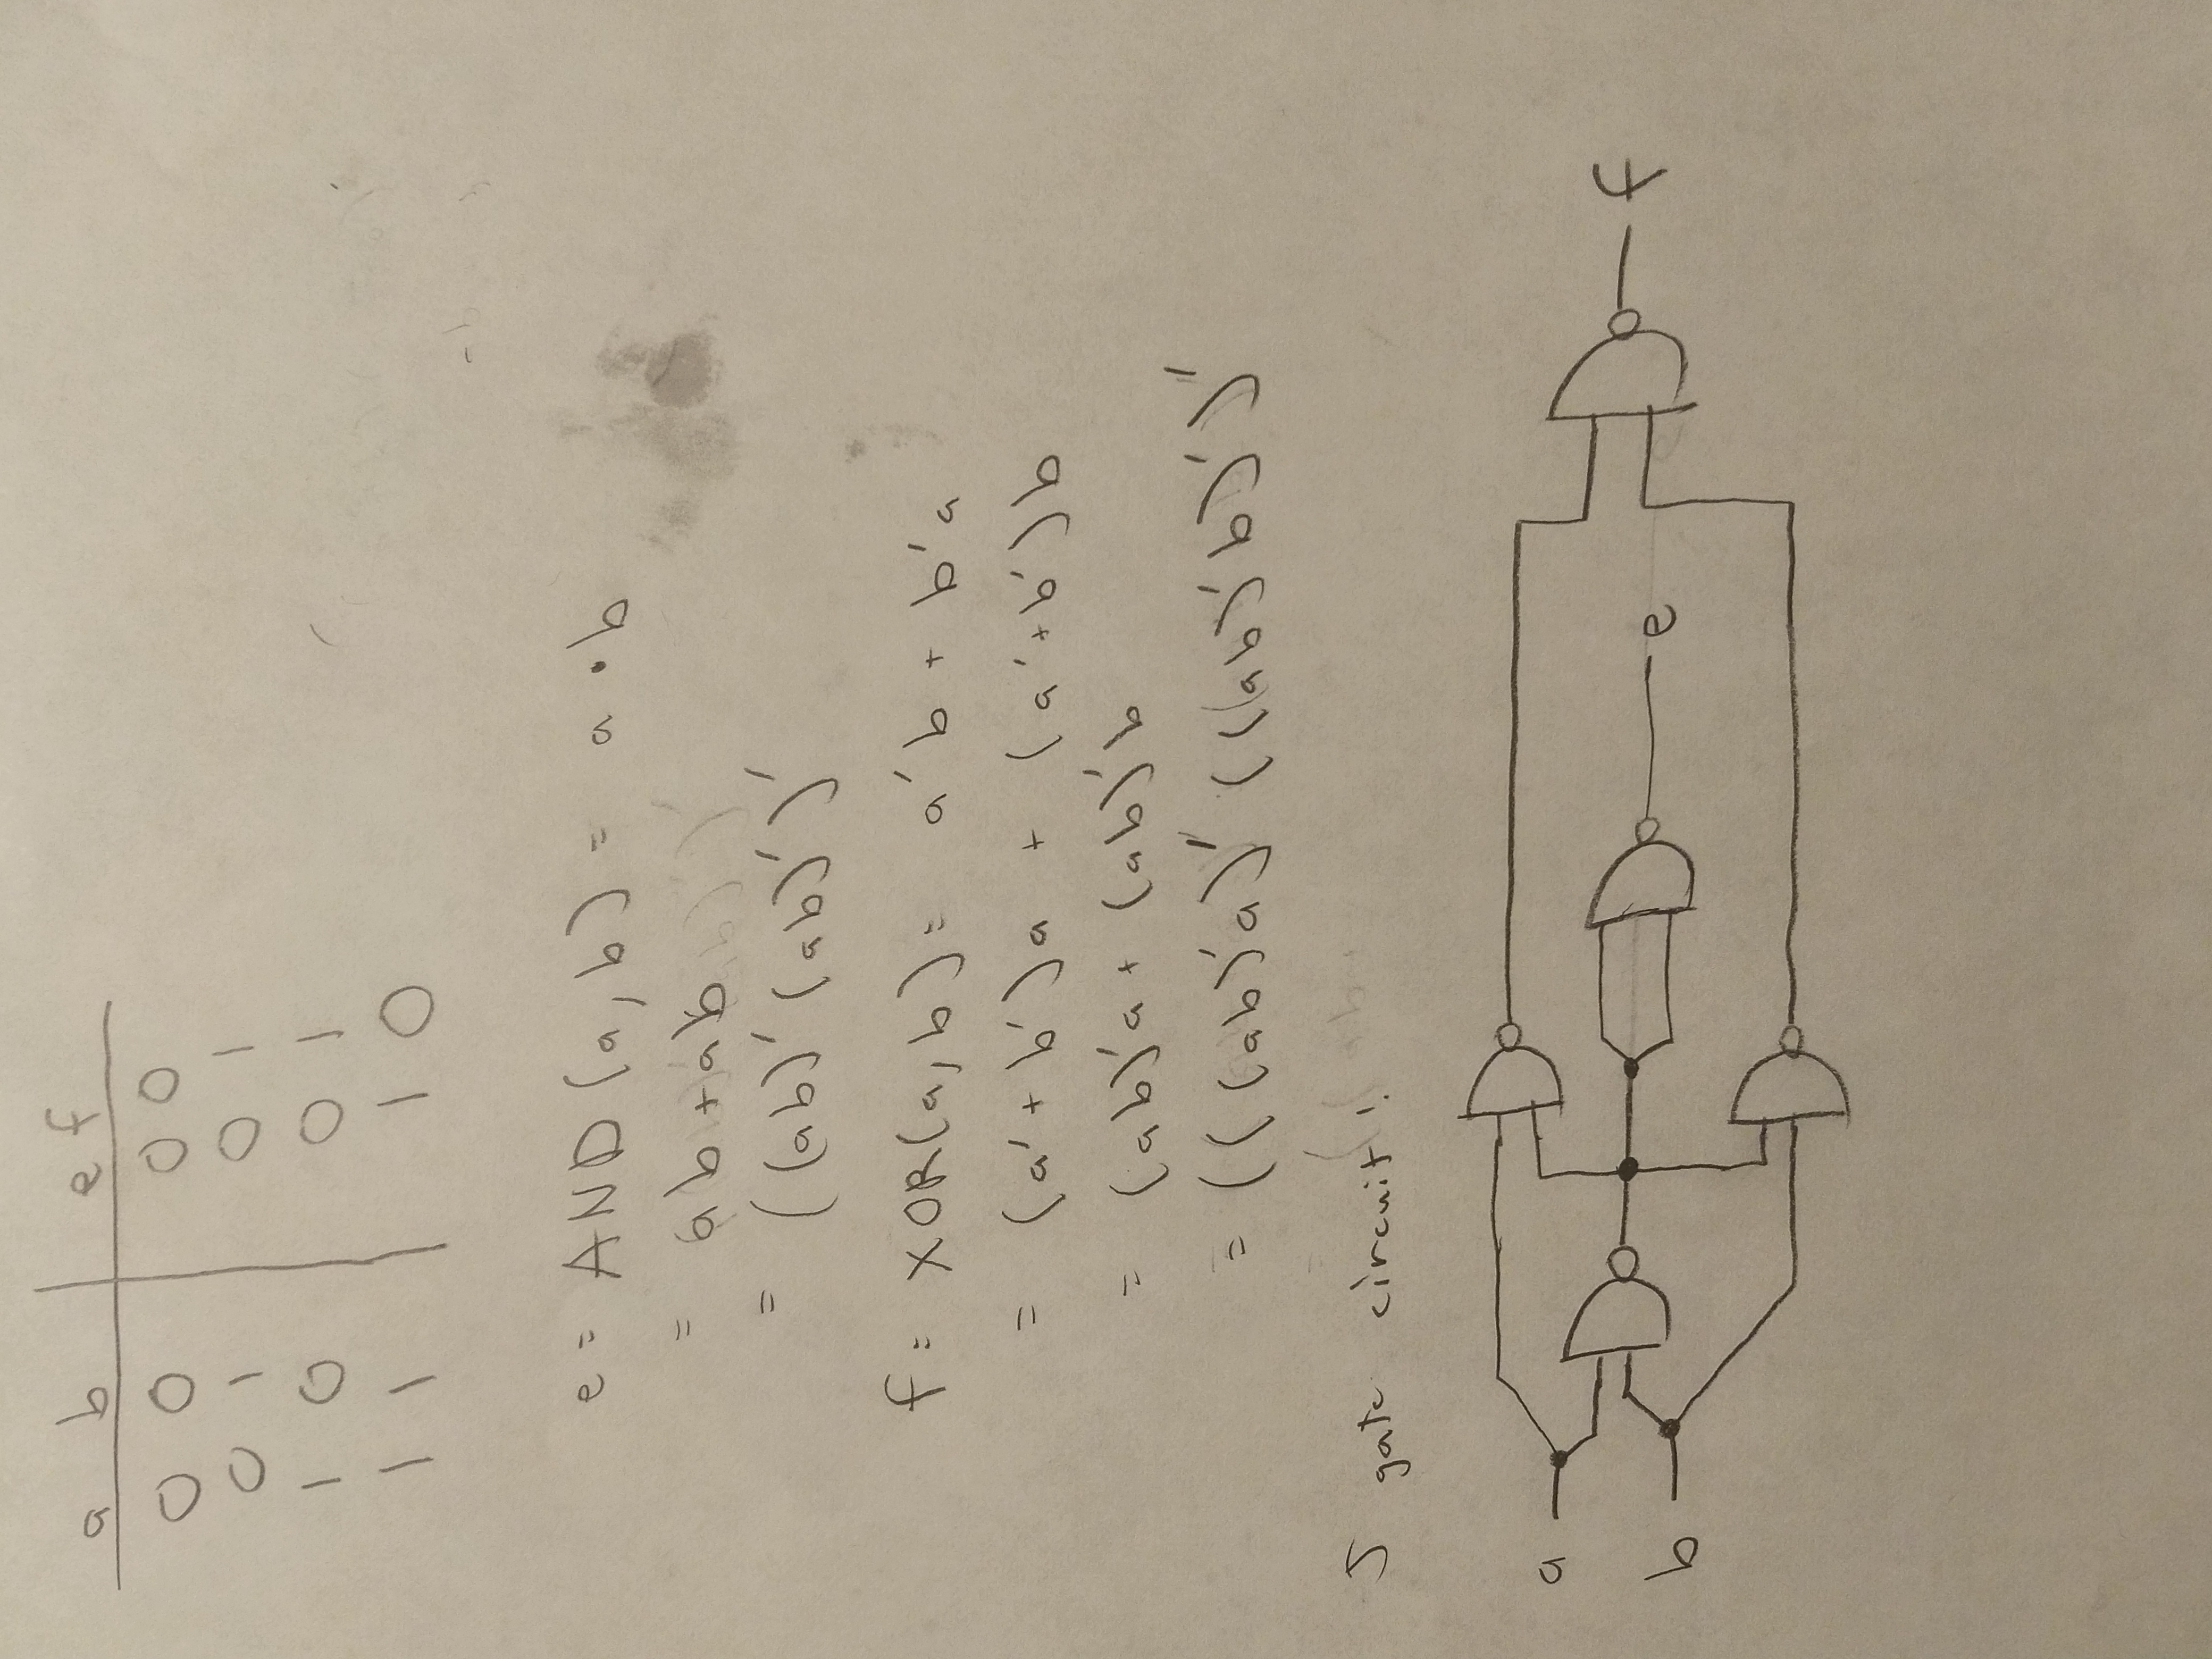
\includegraphics[scale=0.15, angle=-90]{problem1_1.jpg}
\subsection*{Part 2}
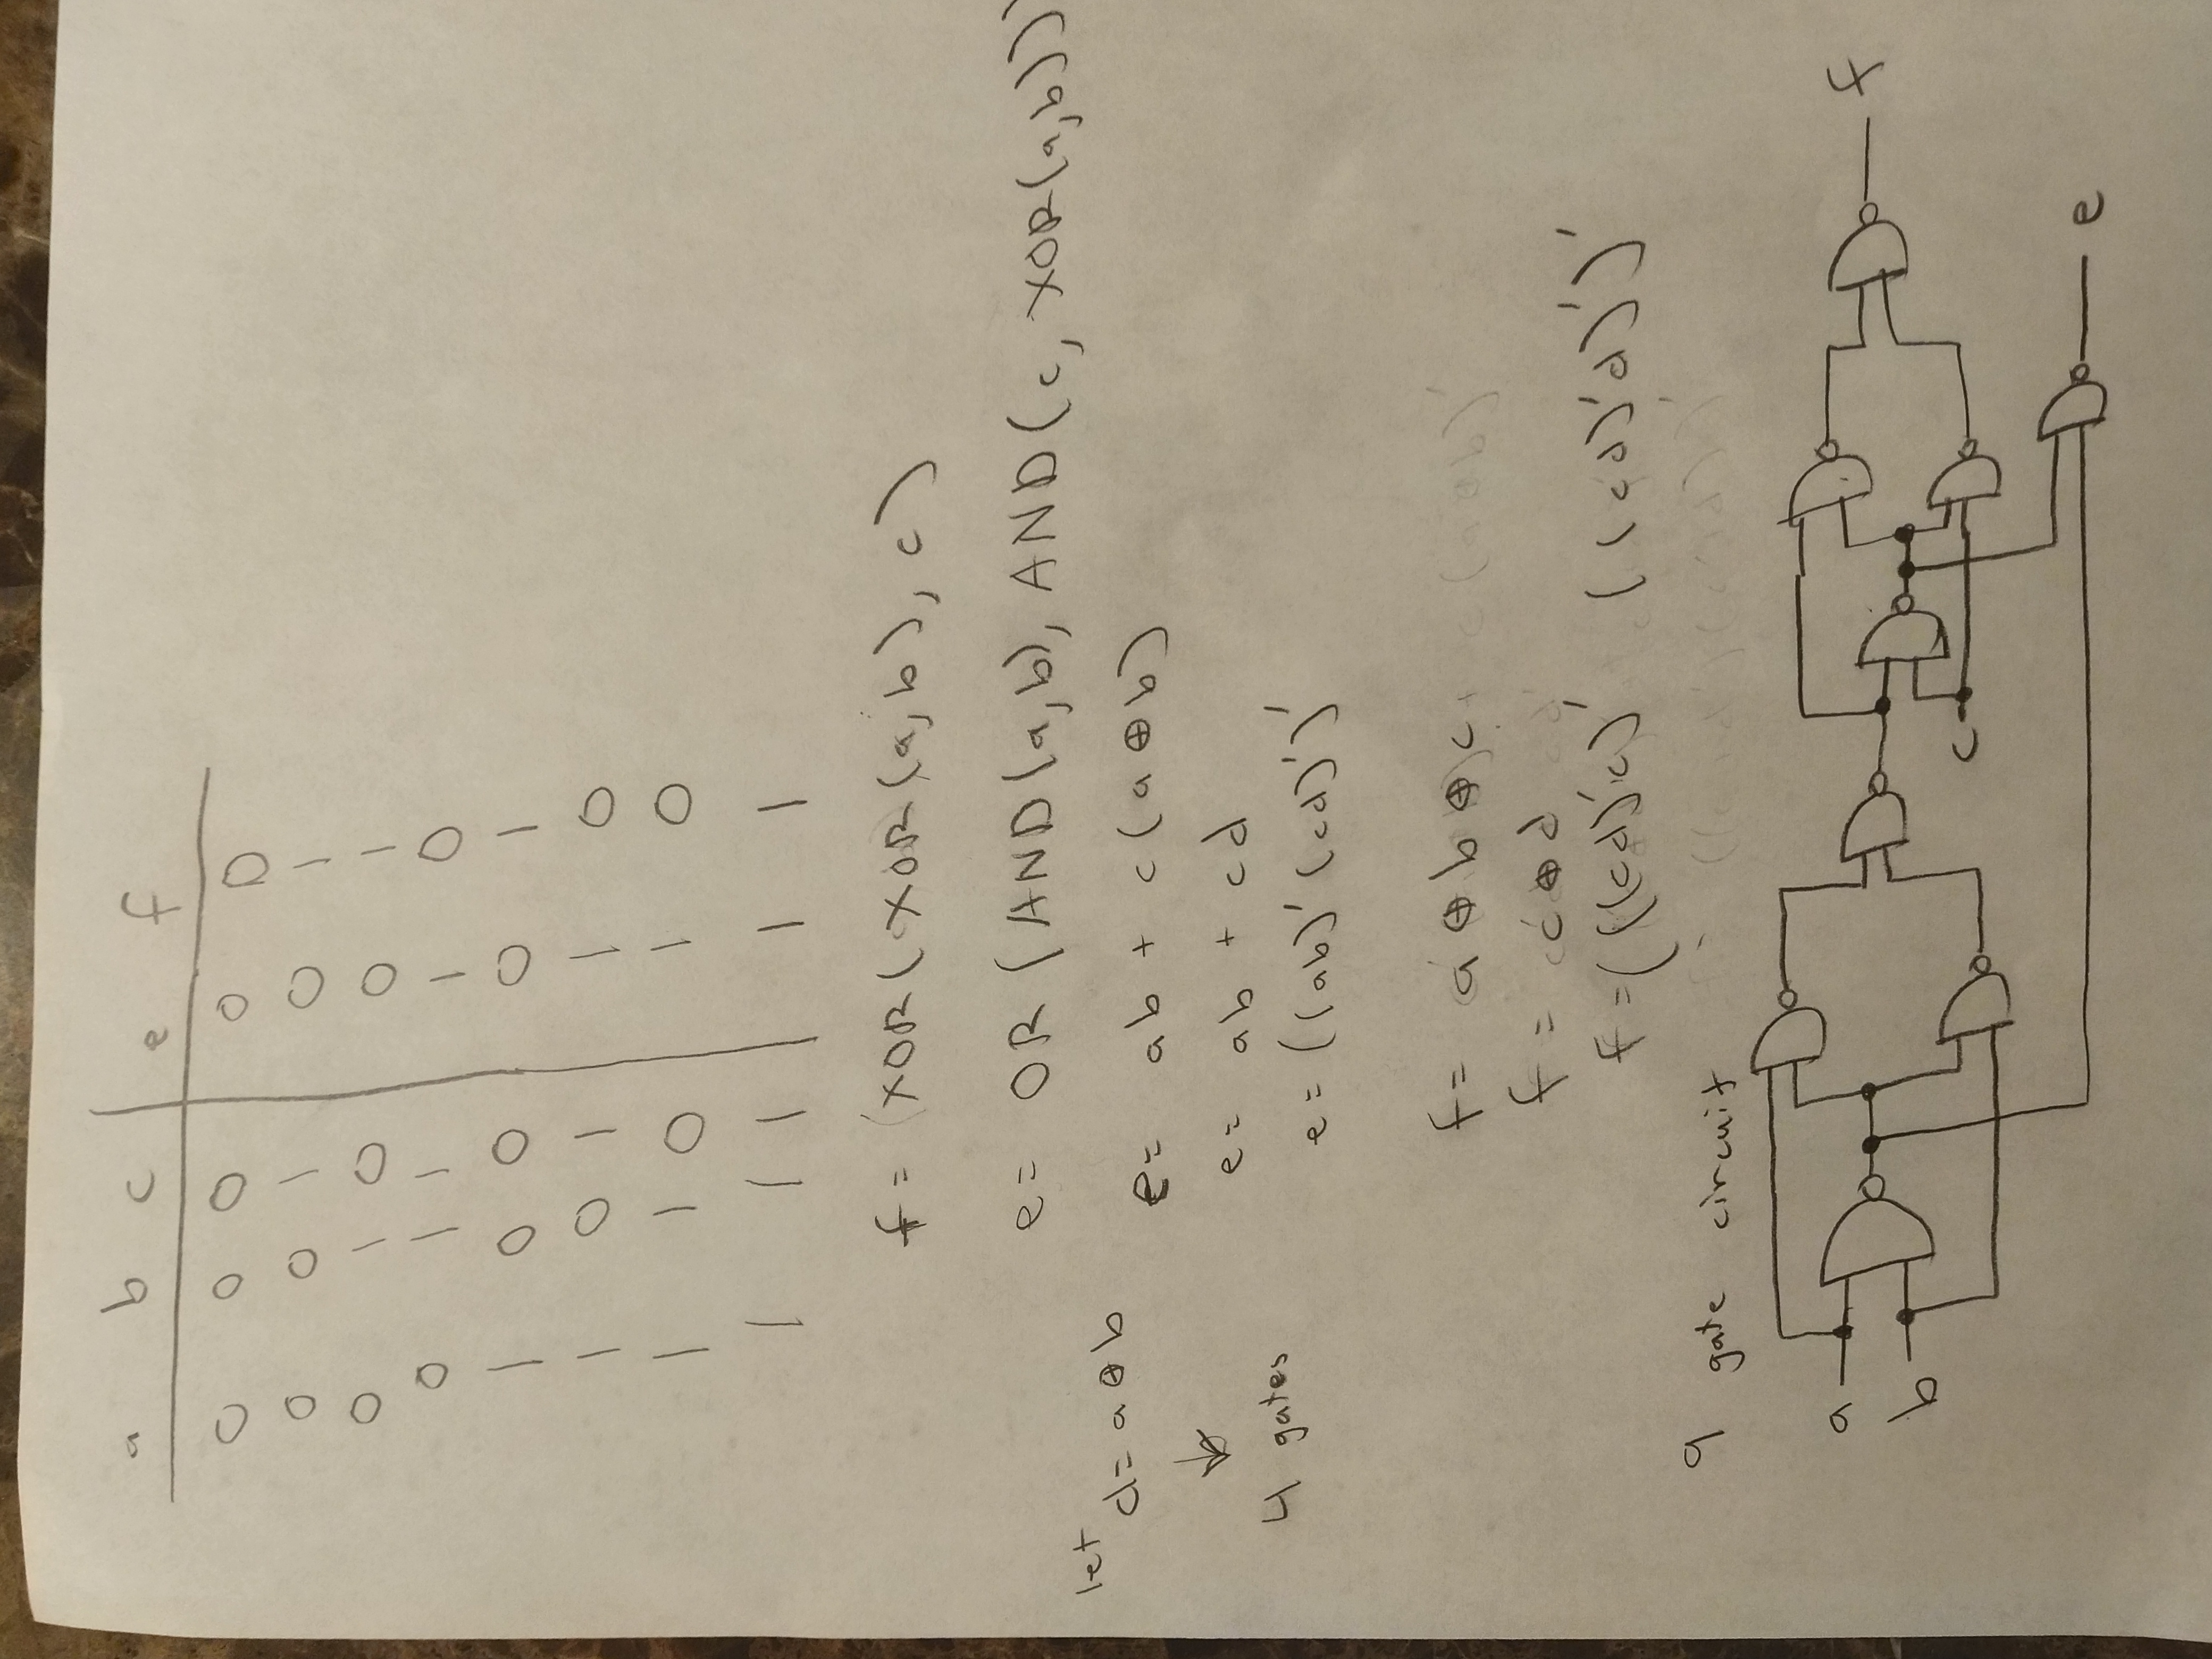
\includegraphics[scale=0.15, angle=-90]{problem1_2.jpg}
\subsection*{Part 3}
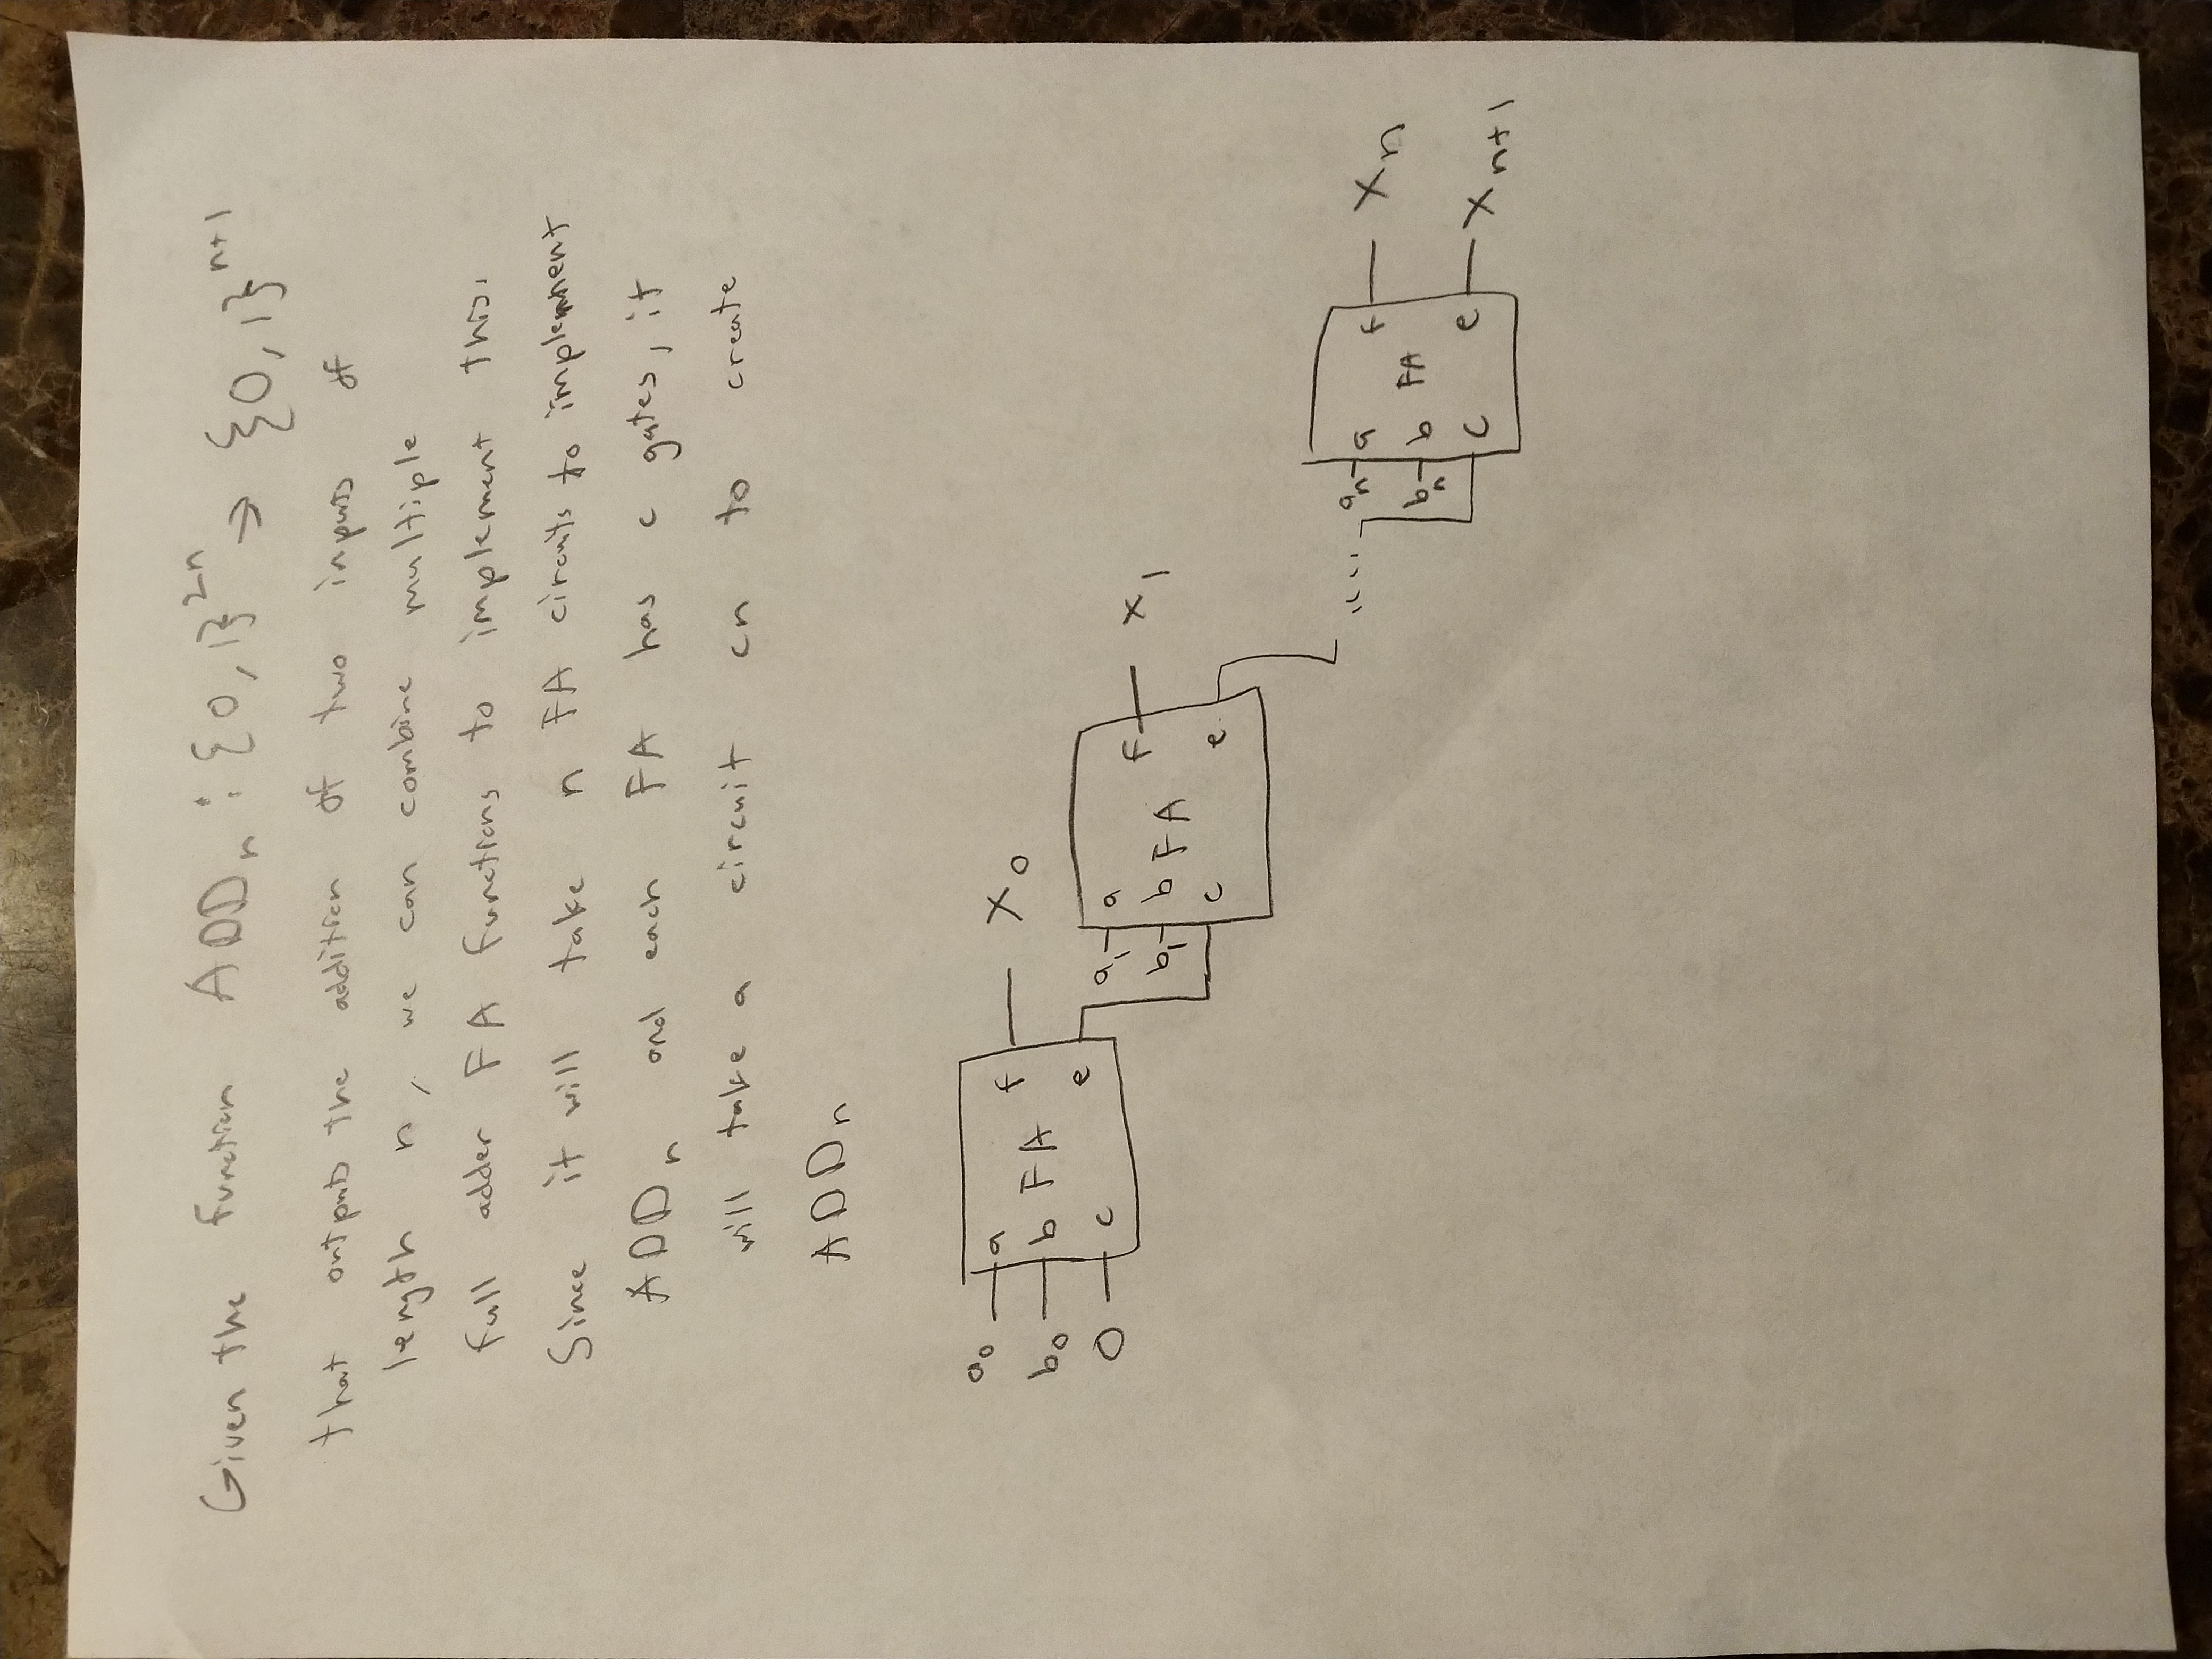
\includegraphics[scale=0.15, angle=-90]{problem1_3.jpg}

\newpage
\section*{Problem 2}
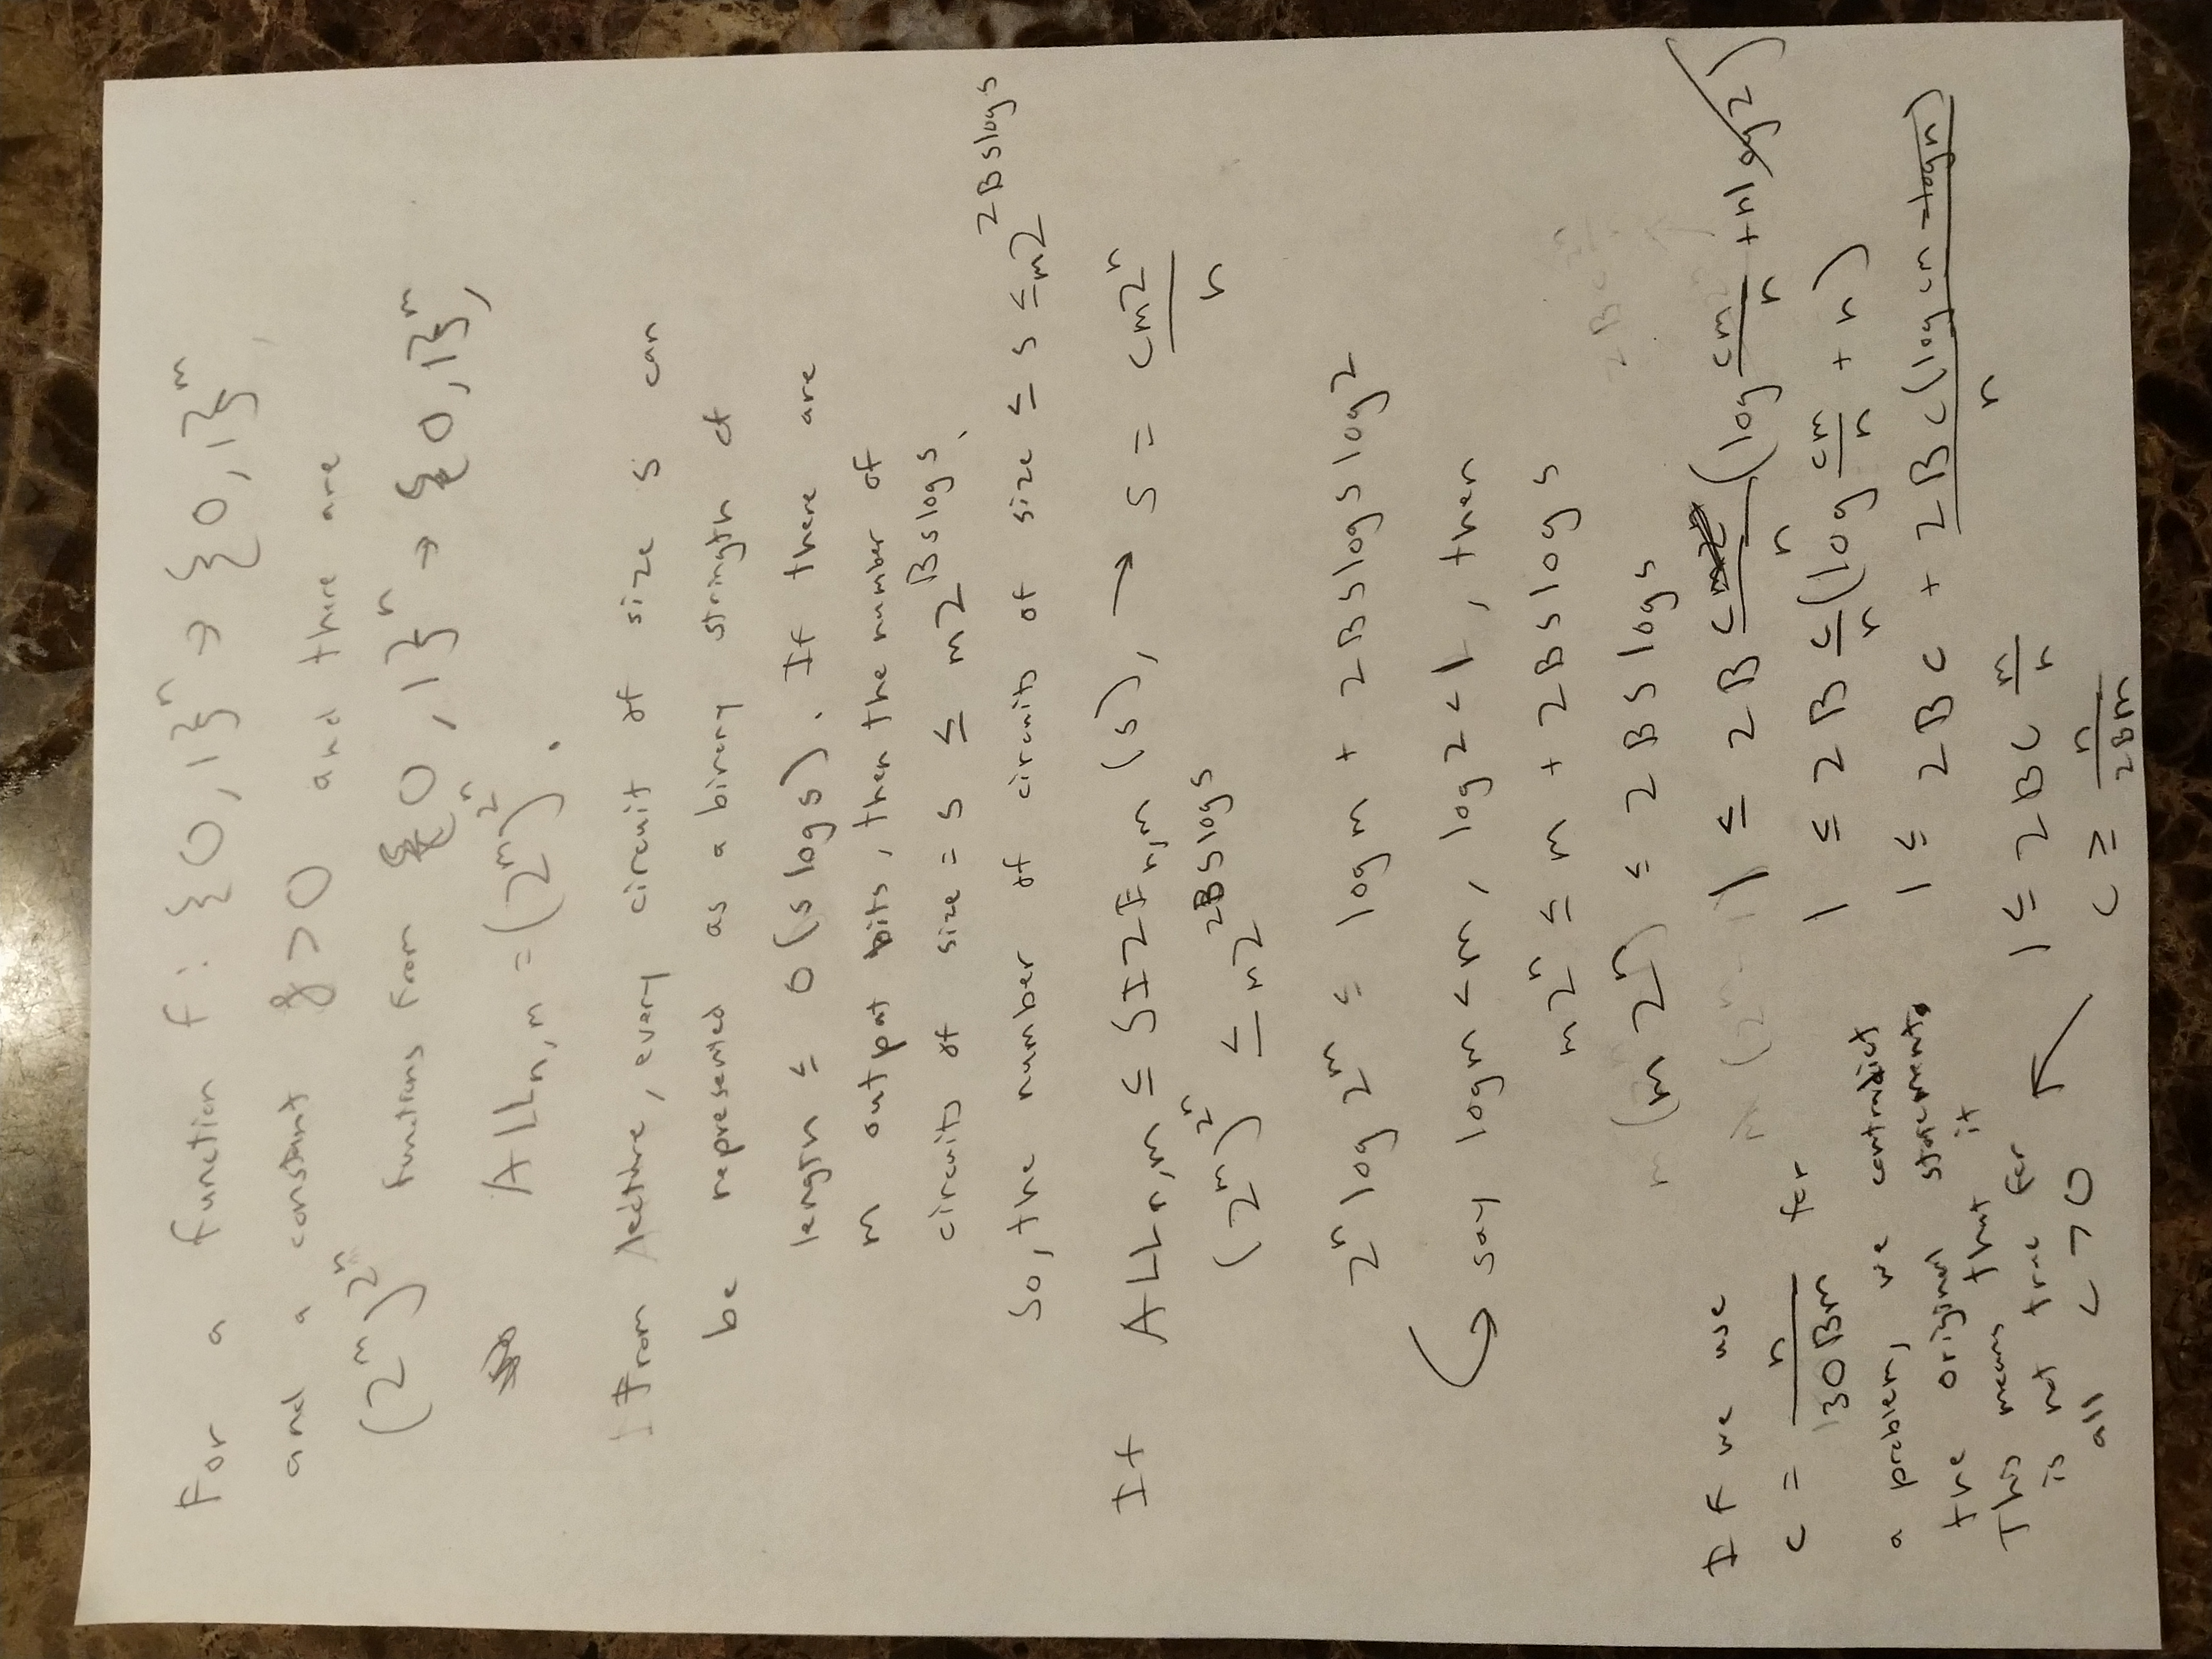
\includegraphics[scale=0.15, angle=-90]{problem2.jpg}

\newpage
\section*{Problem 3}
\subsection*{Part A}
0
\subsection*{Part B}
\{3\}
\subsection*{Part C}
0, 1, 3, 2, 2, 2, 2
\subsection*{Part D}
No, it does not accept the string 010111
\subsection*{Part E}
01

\newpage
\section*{Problem 4}
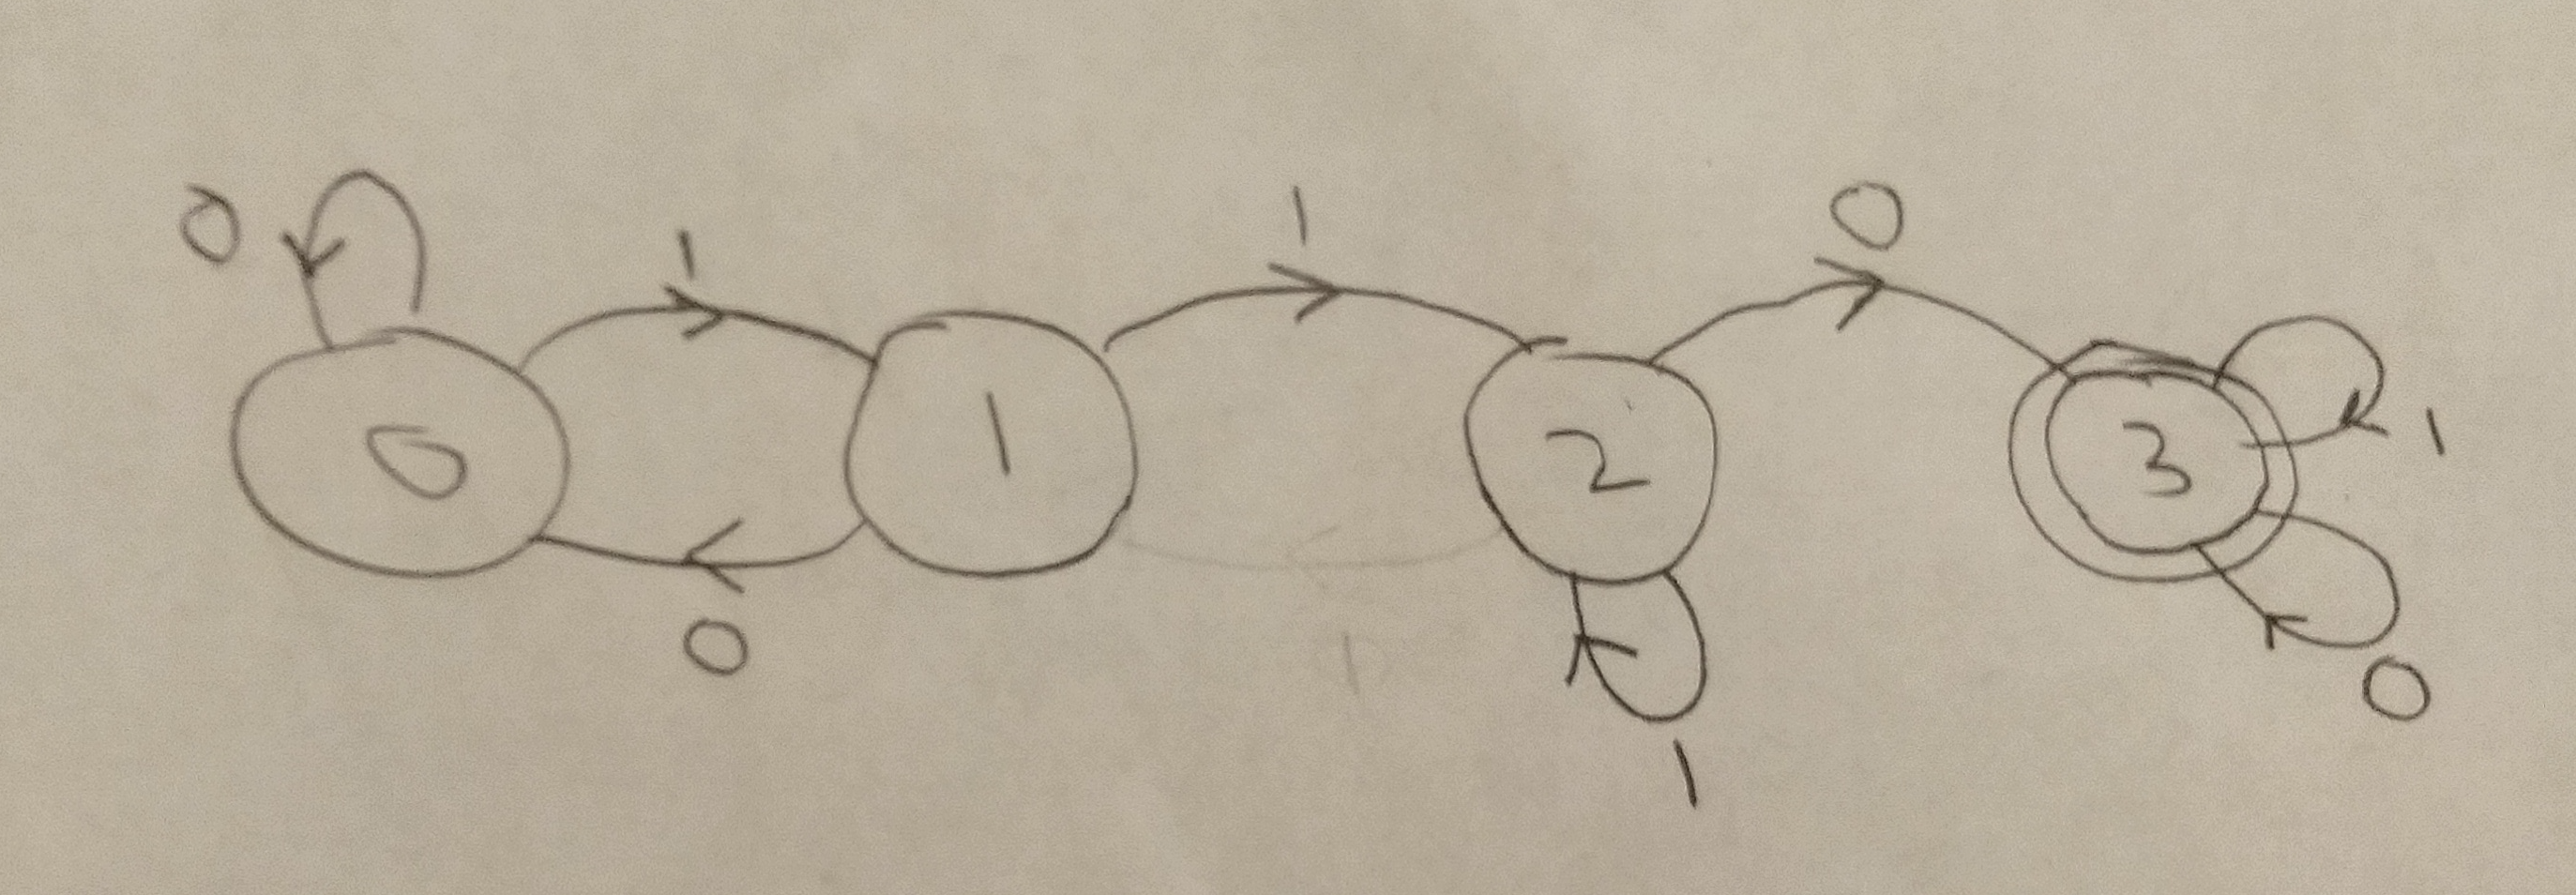
\includegraphics[scale=0.15]{problem4.png}

\newpage
\section*{Problem 5}
It is not possible to have a DFA that will accept strings with more 1's than 0's. An attempt
would be to have 3 main states, a nuetral state, a state that means more 0's than 1's, and 
a state that means more 1's than 0's. However, this does not work because this three state system
does not take into account of a difference of 1's and 0's of more than 1. This means that we would
theoretically need an infinite amount of states in order to act as a weight. 

\end{document}